\subsection{Lyskryds oversigt}
	Dette afsnit vil indeholde en gennem gang af design, grafisk bruger interface og implentering af Lyskryds oversigt activityen til android applikationen
	\subsubsection{Design}
	I dette afsnit ses et design Lyskryds oversigten til android applikationen
	\begin{figure} [!ht]
		\begin{center}
			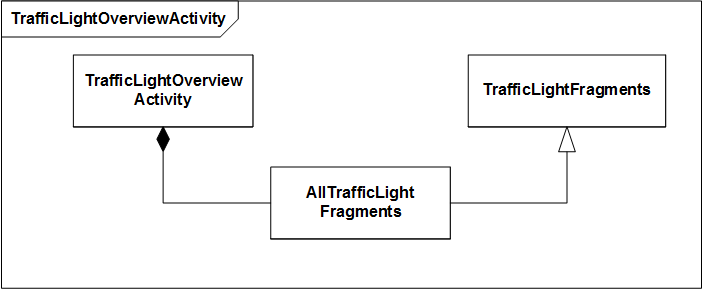
\includegraphics[height=7cm]{Android/Billeder/Lyskryds}
		\end{center}
		\caption{Design over lyskryds oversigten på android applikationen}
		\label{fig:Design over lyskryds oversigten på android applikationen}
	\end{figure}\\
	TrafficLightOverviewActivity er bygget op om samme design som HomeActivity, se figur \vref{fig: Traffic Control - Home Page}. Forskellen mellem Home- og TrafficLightOverviewActivity ligger i at de tabs HomeActivity havde er fjernet. Men derimod har TrafficLightOverviewActivity fået tilføjet et felt hvor du kan vælge en værdi du ønsker at sortere lyskrydsene efter.
	
	\pagebreak
	
	\subsubsection{Grafisk Bruger Interface}	
	\begin{figure} [!ht]
		\begin{center}
			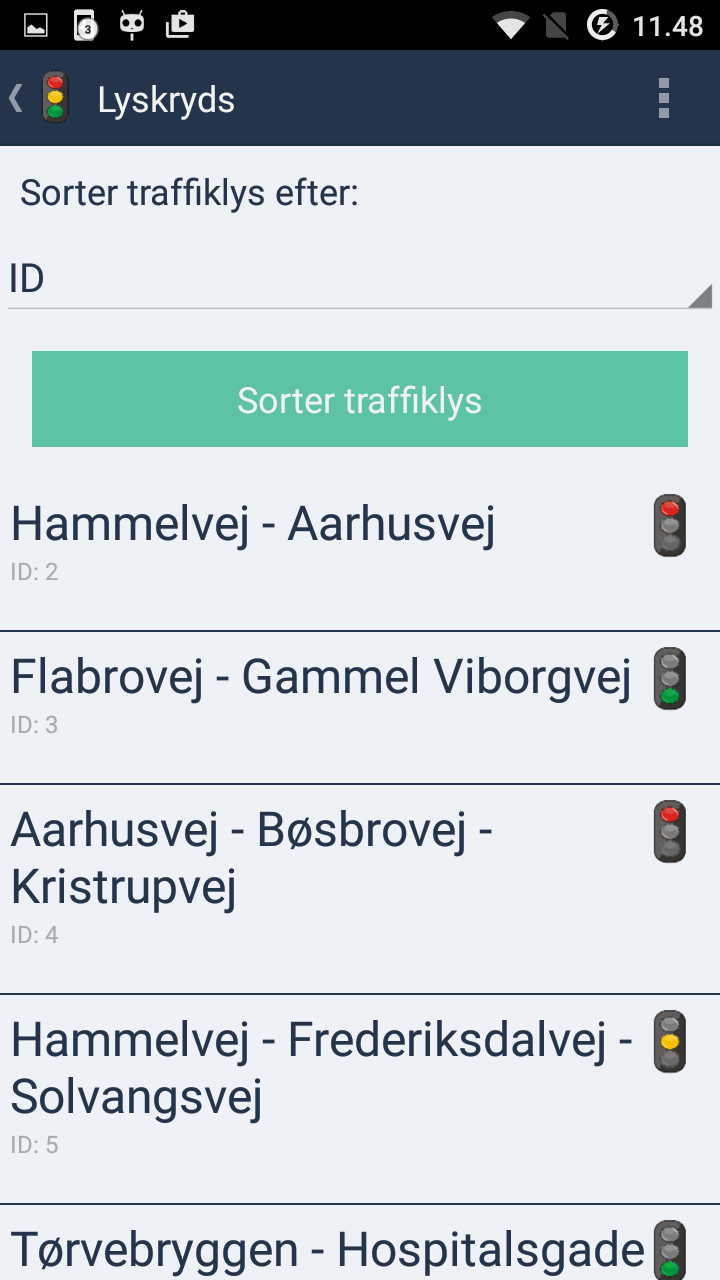
\includegraphics[height=10cm]{Android/Billeder/AndroidLyskryds}
		\end{center}
		\caption{Oversigt over lyskryds på android applikationen}
		\label{fig:Oversigt over lyskryds på android applikationen}
	\end{figure}
	
	\noindent Denne activity i applikationen bruges til at få et overblik over alle lyskryds som der er i databasen. Man kan sortere alle lyskryds efter; adresse, ID eller status. Man kan se om der er en sag på et lyskryds ud fra ikonet ud for en sag, der viser rød eller gul hvis der er en sag der skal have opmærksomhed, eller grøn hvis lyskrydset ingen sager har.\\
	Her fra vil man kunne navigere videre til de enkelte lyskryds, hvorfra man kan se lyskryds' status, placering, log og bilag.
	
	\subsubsection{Implementering}
	Modellen indeholder alle de lyskryds der er i Randers kommune, disse hentes fra DAL-laget.
	Der er øverst i TrafficLightOverviewActivity lavet en spinner samt en knap som gør det muligt at vælge en værdi som ønskes lyskryds sorteret efter.
	Under sorterings delen af activityen består af to fragments som i Homeactivityen, se \vref{HomePageImp}.
	
	
	\pagebreak